\documentclass[]{article}
\usepackage{lmodern}
\usepackage{amssymb,amsmath}
\usepackage{ifxetex,ifluatex}
\usepackage{fixltx2e} % provides \textsubscript
\ifnum 0\ifxetex 1\fi\ifluatex 1\fi=0 % if pdftex
  \usepackage[T1]{fontenc}
  \usepackage[utf8]{inputenc}
\else % if luatex or xelatex
  \ifxetex
    \usepackage{mathspec}
  \else
    \usepackage{fontspec}
  \fi
  \defaultfontfeatures{Ligatures=TeX,Scale=MatchLowercase}
\fi
% use upquote if available, for straight quotes in verbatim environments
\IfFileExists{upquote.sty}{\usepackage{upquote}}{}
% use microtype if available
\IfFileExists{microtype.sty}{%
\usepackage{microtype}
\UseMicrotypeSet[protrusion]{basicmath} % disable protrusion for tt fonts
}{}
\usepackage[margin=1in]{geometry}
\usepackage{hyperref}
\hypersetup{unicode=true,
            pdftitle={MAthesis},
            pdfauthor={Julia Joos},
            pdfborder={0 0 0},
            breaklinks=true}
\urlstyle{same}  % don't use monospace font for urls
\usepackage{natbib}
\bibliographystyle{plainnat}
\usepackage{longtable,booktabs}
\usepackage{graphicx,grffile}
\makeatletter
\def\maxwidth{\ifdim\Gin@nat@width>\linewidth\linewidth\else\Gin@nat@width\fi}
\def\maxheight{\ifdim\Gin@nat@height>\textheight\textheight\else\Gin@nat@height\fi}
\makeatother
% Scale images if necessary, so that they will not overflow the page
% margins by default, and it is still possible to overwrite the defaults
% using explicit options in \includegraphics[width, height, ...]{}
\setkeys{Gin}{width=\maxwidth,height=\maxheight,keepaspectratio}
\IfFileExists{parskip.sty}{%
\usepackage{parskip}
}{% else
\setlength{\parindent}{0pt}
\setlength{\parskip}{6pt plus 2pt minus 1pt}
}
\setlength{\emergencystretch}{3em}  % prevent overfull lines
\providecommand{\tightlist}{%
  \setlength{\itemsep}{0pt}\setlength{\parskip}{0pt}}
\setcounter{secnumdepth}{5}
% Redefines (sub)paragraphs to behave more like sections
\ifx\paragraph\undefined\else
\let\oldparagraph\paragraph
\renewcommand{\paragraph}[1]{\oldparagraph{#1}\mbox{}}
\fi
\ifx\subparagraph\undefined\else
\let\oldsubparagraph\subparagraph
\renewcommand{\subparagraph}[1]{\oldsubparagraph{#1}\mbox{}}
\fi

%%% Use protect on footnotes to avoid problems with footnotes in titles
\let\rmarkdownfootnote\footnote%
\def\footnote{\protect\rmarkdownfootnote}

%%% Change title format to be more compact
\usepackage{titling}

% Create subtitle command for use in maketitle
\newcommand{\subtitle}[1]{
  \posttitle{
    \begin{center}\large#1\end{center}
    }
}

\setlength{\droptitle}{-2em}
  \title{MAthesis}
  \pretitle{\vspace{\droptitle}\centering\huge}
  \posttitle{\par}
  \author{Julia Joos}
  \preauthor{\centering\large\emph}
  \postauthor{\par}
  \predate{\centering\large\emph}
  \postdate{\par}
  \date{14 August 2017}

\usepackage{setspace}
\doublespacing

\begin{document}
\maketitle

\begin{longtable}[]{@{}llrrrr@{}}
\caption{Time bins with age range, mean age, epoch name and
corresponding sample sizes (on individual, species and genus
level)}\tabularnewline
\toprule
bin & EpochBins & MeanBins & nIndividuals & nSpecies &
nGenera\tabularnewline
\midrule
\endfirsthead
\toprule
bin & EpochBins & MeanBins & nIndividuals & nSpecies &
nGenera\tabularnewline
\midrule
\endhead
(0,1e-06{]} & Modern & 0.0000005 & 240 & 58 & 18\tabularnewline
(0.0117,0.126{]} & Upper Pleistocene & 0.0688500 & 46 & 15 &
7\tabularnewline
(0.126,0.781{]} & Middle Pleistocene & 0.4535000 & 46 & 9 &
6\tabularnewline
(0.781,2.59{]} & Lower Pleistocene & 1.6845000 & 68 & 24 &
11\tabularnewline
(1e-06,0.0117{]} & Holocene & 0.0058500 & 12 & 6 & 4\tabularnewline
(2.59,3.6{]} & Upper Pliocene & 3.0940000 & 21 & 14 & 9\tabularnewline
(3.6,5.33{]} & Lower Pliocene & 4.4660000 & 27 & 16 & 8\tabularnewline
(5.33,11.6{]} & Upper Miocene & 8.4700000 & 41 & 21 & 9\tabularnewline
\bottomrule
\end{longtable}

\begin{figure}[htbp]
\centering
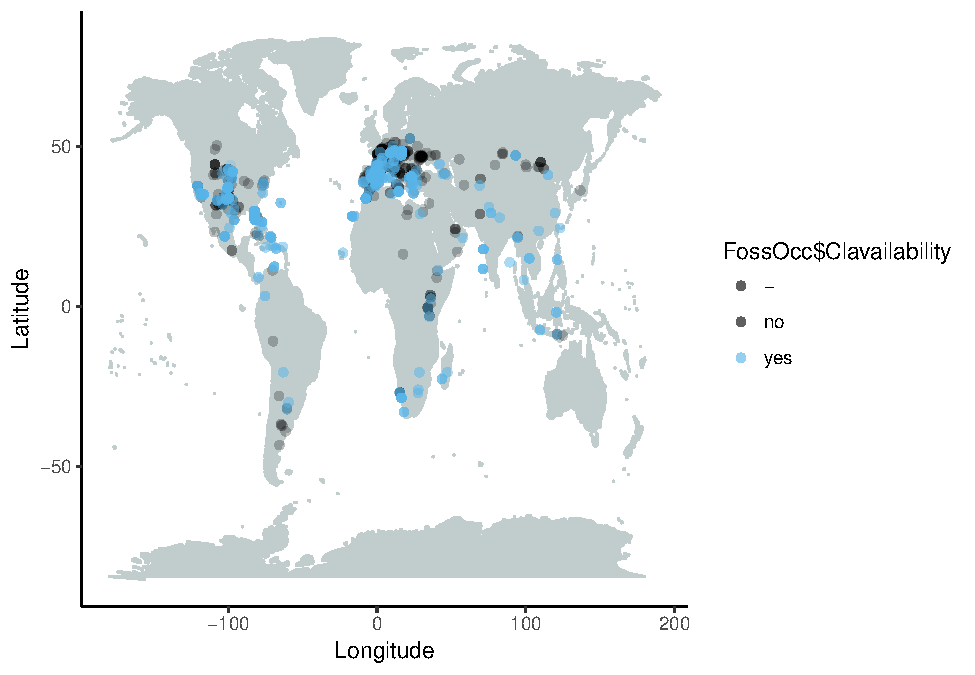
\includegraphics{MA_JJ_files/figure-latex/Map fossil occurrences-1.pdf}
\caption{Map displaying all fossil occurrences of testudinids, with
color indicating whether relevant literature was available (black if
not) and if it was, whether body size data was available or not (yes and
no, respectively).}
\end{figure}

\begin{figure}[htbp]
\centering
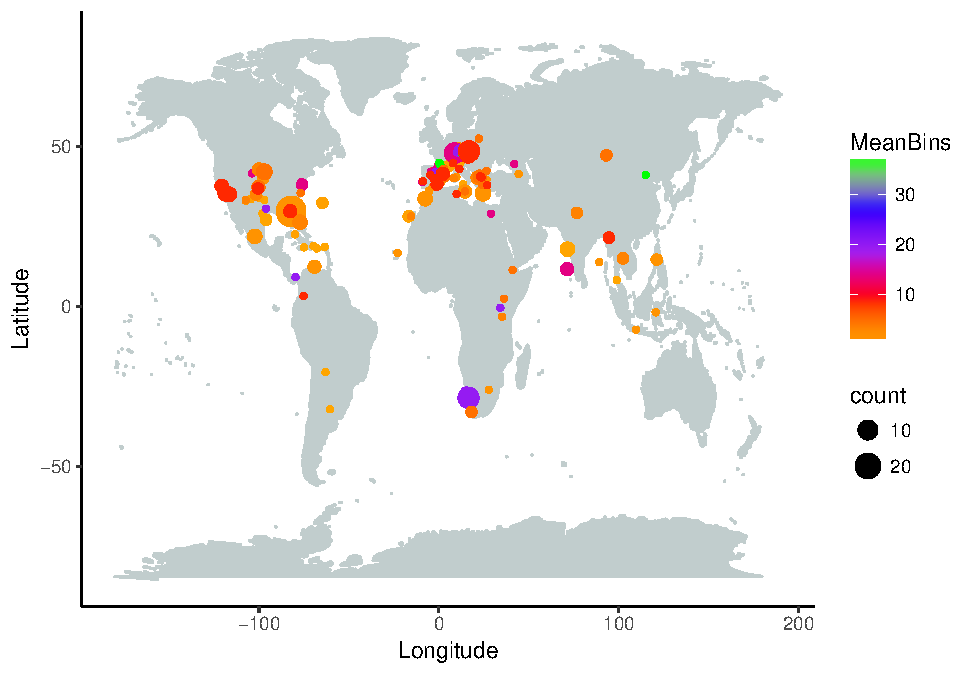
\includegraphics{MA_JJ_files/figure-latex/Map body size data set-1.pdf}
\caption{Map displaying all localities for which body size data for
testudinids was available in the literature. Size of points denotes
sample size, color denotes approximate age.}
\end{figure}


\end{document}
